%!TEX root = main.tex
\documentclass
[
	a4paper,
	11pt,				% 10pt, 11pt oder 12pt - Standard ist 10pt
	pointlessnumbers,	% kein abschlie�enden Punkt hinter den Nummerierungen machen
	%pdftex,
	%chapterprefix,		% Kapitel anschreiben als Kapitel
	%openright, 		
	%openany,
	twoside,
	abstracton,
	final,				%draft,
	%normalheadings,	% �berschriften etwas kleiner (smallheadings)
	%BCOR21mm,			% Bindekorrektur, bspw. 1 cm
	%DIV13,			% f�hrt die Satzspiegelberechnung neu aus
	bibtotoc			% Literaturverzeichniss in toc eintragen
	%bibgerm,			% wegen BibTex in Deutschen Stil, sollte an alle weitergegeben werden
]
{scrreprt}				% KOMA-Script 

%\pagestyle{headings}			% sieht gut aus

% Packages:
%\usepackage[ngerman]{babel}
\usepackage[USenglish]{babel}
\usepackage[T1]{fontenc}		% f�r T1 Zeichensatz
\usepackage{lmodern} 			% Type1-Schriftart f�r nicht-englische Texte

\usepackage{amsmath}
\usepackage{amsthm}
\usepackage{amssymb}
%\usepackage{dsfont}				% brauche ich bis jetzt nur f�r die Zahlenbereiche: N,R,Z 
%\usepackage[babel,german=quotes]{csquotes}	% f�r einheitliche Anf�hrungszeichen

\usepackage{tikz}		% syntax layer for pgf, a tae macro package for generating graphics
\usetikzlibrary{plotmarks}
\usepackage{verbatim}

%\usetikzlibrary{chains,decorations}
\usepackage{pgf}
\usepackage{xcolor}				% f�r Farbmischungen
\usepackage{multicol}			% f�r mehrere Spalten
\usepackage{url}	
\usepackage{nameref}			% um Kapitel�berschriften referenzieren zu k�nnen

%\renewcaptionname{ngerman}{\abstractname}{Kurzfassung}

%\usepackage{caption}	% ich mache lieber alles �ber das Koma Script:
	\setcapindent{0em}	% kein Einzug
	\addtokomafont{caption}{\footnotesize} %\footnotesize \small 
	\addtokomafont{captionlabel}{\sffamily\bfseries}

%% Packages f�r Grafiken & Abbildungen %%%%%%%%%%%%%%%%%%%%%%
\usepackage{graphicx} %%Zum Laden von Grafiken
\usepackage{subfig} %%Teilabbildungen in einer Abbildung
\usepackage{float}		% f�r den [H] exakt hier Specifier
\usepackage{pdfpages}



% wichtig: hyperef muss als letztes Paket geladen werden, weiter Optionen: [pdfstartview={Fit}, pagebackref]
%\xdefinecolor{urlFarbe}{rgb}{0.0,0.5,0.5}
\usepackage[pdfauthor={Fabian Langguth}, bookmarks=false, pdftex, colorlinks=true, urlcolor=urlFarbe, linkcolor=black, citecolor=black]{hyperref}


%\areaset[66pt]{415pt}{600pt}


\begin{document}
\title{WEKA Projekt}
\author{Fabian Langguth, Sebastian Koch}
\date{Wintersemester 10/11}

\maketitle

%TODO formatieren!
\section*{Aufgabe 1 Regellernen} 

F\"ur diese Aufgabe benutzen wir die Datens\"atze \emph{glass, iris} und \emph{splice}.
\emph{glass} wurde f\"ur den Prism-Learner mit dem Discretize-Filter verwendet (\emph{java weka.filters.supervised.attribute.Discretize -i glass.arff -o glass\_nom.arff -R 1,2,3,4,5,6,7,8,9 -c last}).\\

Anzahl der Regeln \\
\begin{tabular}{c|c|c|c}
	             & glass & iris & splice \\ \hline
Conjunctive Rule &   1   &  1   &   1    \\ \hline
JRip             &   8   &  4   &   14   \\ \hline
Prism	         &   63  &  16   &  3176    \\
\end{tabular}\\ \\

Gesamtanzahl der Bedingungen \\
\begin{tabular}{c|c|c|c}
	             & glass & iris & splice \\ \hline
Conjunctive Rule &   2   &  1   &   1    \\ \hline
JRip             &  18   &  3   &   55   \\ \hline
Prism	         &  385  & 51   &   3176   \\
\end{tabular}\\ \\

Anzahl der vorhergesagten Klassen \\
\begin{tabular}{c|c|c|c}
	             & glass & iris & splice \\ \hline
Conjunctive Rule &   1   &  1   &   1    \\ \hline
JRip             &   6   &  3   &   3    \\ \hline
Prism	         &   6   &  3   &   3    \\
\end{tabular}\\ \\


Eine Default Rule existiert nur bei JRip. Dort wird als Defaultklasse \"ublicherweise die Klasse gew\"ahlt, die am h\"aufigsten im Datensatz vorkommt. 

Der Datensatz \emph{iris} l\"asst sich am einfachsten lernen, da man hier besonders wenig Regeln und besonders wenig Bedingungen ben\"otigt.

\newpage

\section*{Aufgabe 2 Evaluation von Regellernern}
\subsubsection*{a}
\textbf{Accuracy}
\begin{table}[htb]
	\centering
\begin{tabular}{c|c|c|c|c|c}
				Datensatz         & 1x5  & 1x10 & 1x20 & LOO  & Trainingsmenge   \\ \hline
				\emph{glass}      & 67.3 & 61.8 & 60.7 & 61.7 & 85.98   \\ \hline
				\emph{iris}       & 92.0 & 88.0 & 96.0 & 93.3 & 96.0    \\ \hline
				\emph{audiology}  & 67.3 & 66.4 & 69.9 & 69.9 & 76.1    \\ \hline
				\emph{ionosphere} & 89.2 & 92.0 & 90.0 & 89.2 & 100   \\ \hline
				\emph{yeast}      & 56.5 & 57.7 & 57.7 & 59.4 & 67.8   \\ 
\end{tabular}
\end{table}

Die gesch\"atzte Genauigkeit wird auf der gesamten Trainingsmenge immer h\"oher sein als auf Echtdaten, da die Regeln speziell f\"ur diese Daten trainiert wurden. In der Praxis sollte man daher Cross-Validation verwenden um sinnvolle Genauigkeiten zu erhalten. Die Qualit\"at der Absch\"atzung wird besser, je mehr Folds man f\"ur die Cross-Validation verwendet. Am genauesten sollte die Leave-One-Out Methode sein, sie ben\"otigt jedoch auch die meiste Zeit. In der Praxis sollte man darauf R\"ucksicht nehmen.

\subsubsection*{b}
\begin{table}[htb]
	\centering
\begin{tabular}{c|c}
				Datensatz         & 10x10    \\ \hline
				\emph{glass}      & 67.3     \\ \hline
				\emph{iris}       & 92.0     \\ \hline
				\emph{audiology}  & 67.3     \\ \hline
				\emph{ionosphere} & 89.2     \\ \hline
				\emph{yeast}      & 56.5     \\ 
\end{tabular}
\end{table}

Die \"Anderung des seeds hat keine signifikante Ver\"anderung der Absch\"atzung bewirkt. Im Allgemeinen sollte die Auswahl der Random-Seeds auch keinen Einfluss auf die Absch\"atzung haben.


\subsubsection*{c}
\begin{table}[htb]
	\centering
\begin{tabular}{c|c}
				Datensatz         & Validierungsmenge    \\ \hline
				\emph{glass}      & 73.1     \\ \hline
				\emph{iris}       & 93.3     \\ \hline
				\emph{audiology}  & 67.3   \\ \hline
				\emph{ionosphere} & 84.6   \\ \hline
				\emph{yeast}      & 56.1 \\ 
\end{tabular}
\end{table}

Die Genauigkeit der Evaluierungsmethoden h\"angt stark vom entsprechenden Datensatz ab. Im Allgemeinen konnte keine Methode immer gute Absch\"atzungen liefern.

\newpage

\section*{Aufgabe 3 ROC-Kurven}
Datensatz: glass

\textbf{Fl\"ache unter ROC Kurve}
\begin{table}[htb]
	\centering
\begin{tabular}{c|c|c|c}
				Regellerner       & \emph{build wind float} & \emph{containers} & \emph{tableware}  \\ \hline
				\emph{J48}			& 0.81 & 0.87 & 0.93  \\ \hline
				\emph{Naive Bayes}  & 0.71 & 0.84 & 0.98  
\end{tabular}
\end{table}

\begin{figure}[htbp]
	\centering
		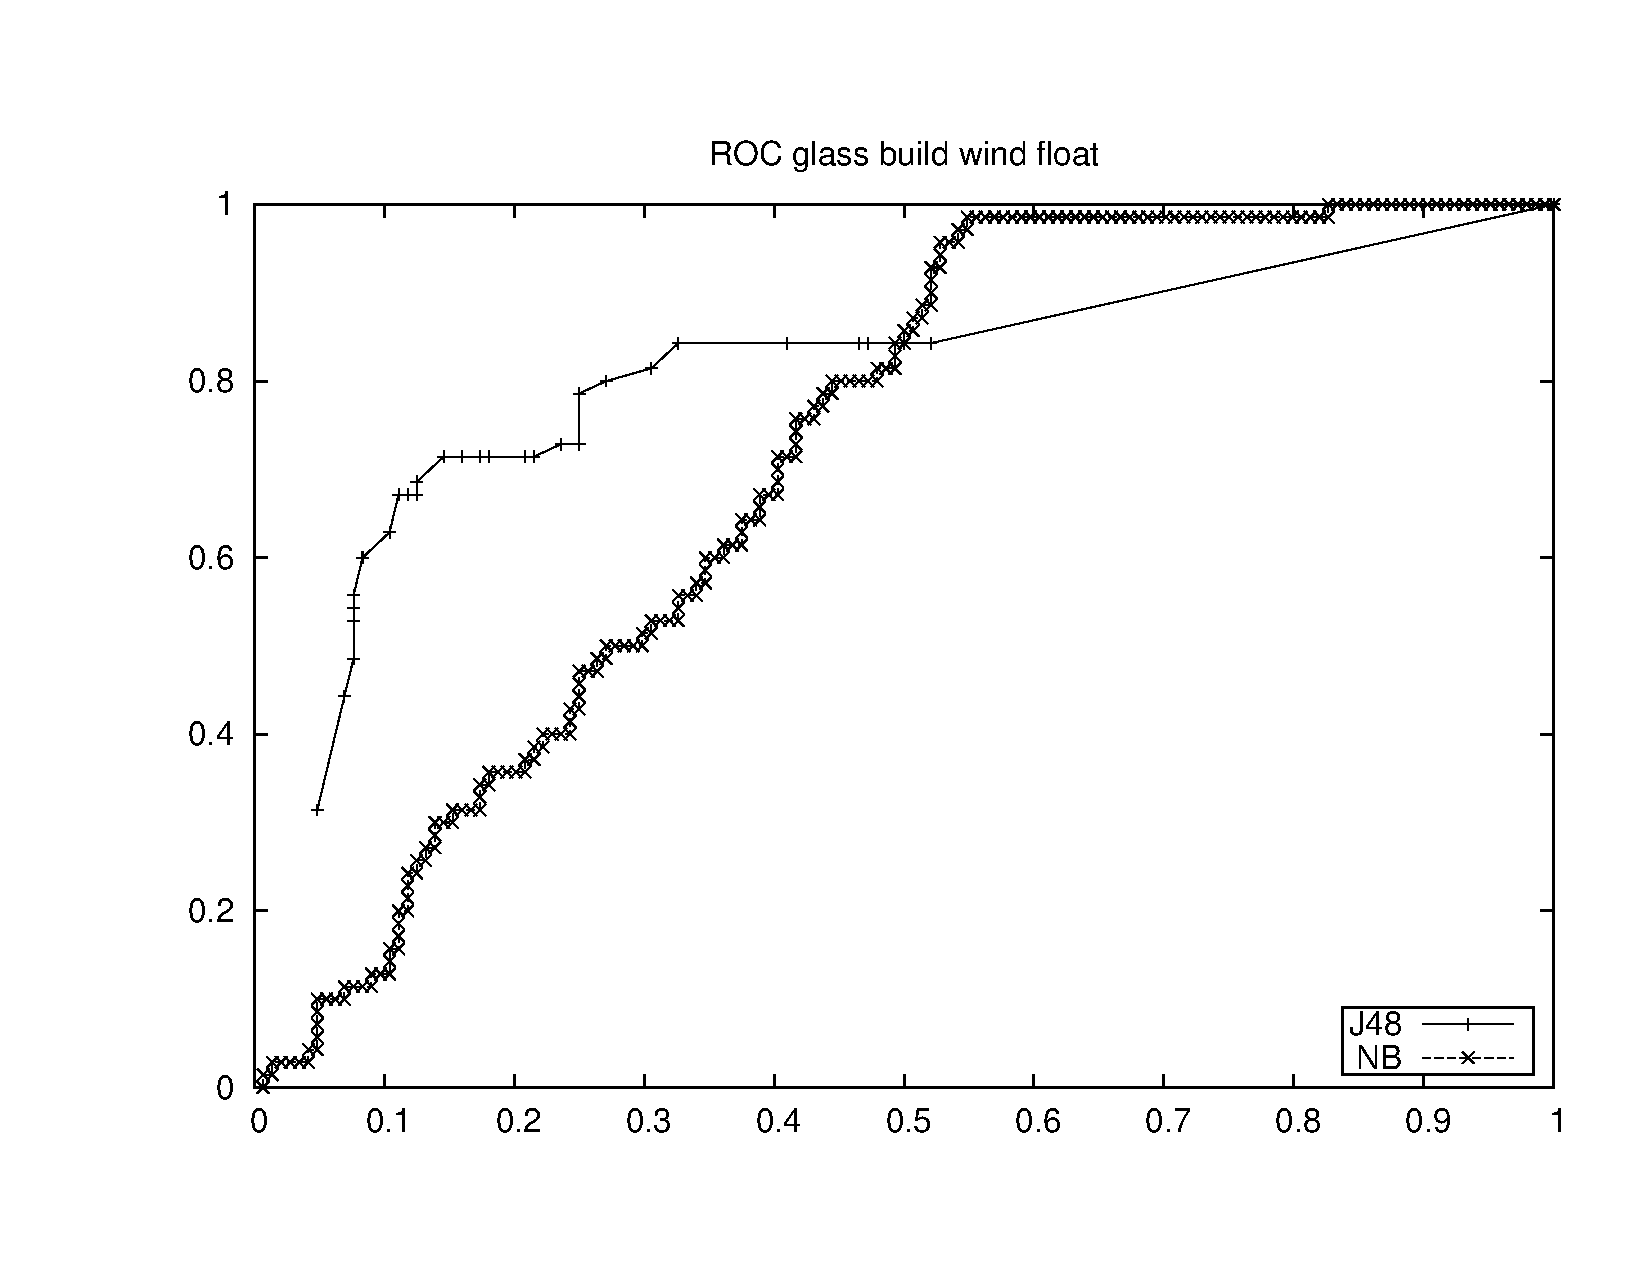
\includegraphics[height=3in]{pics/a3/ROC_glass_build_wind_float.pdf}
	\caption{ROC-Kurve f\"ur \emph{Naive Bayes} und \emph{J48} \"uber das Attribut \emph{build\_wind\_float}}
\end{figure}

\begin{figure}[htbp]
	\centering
		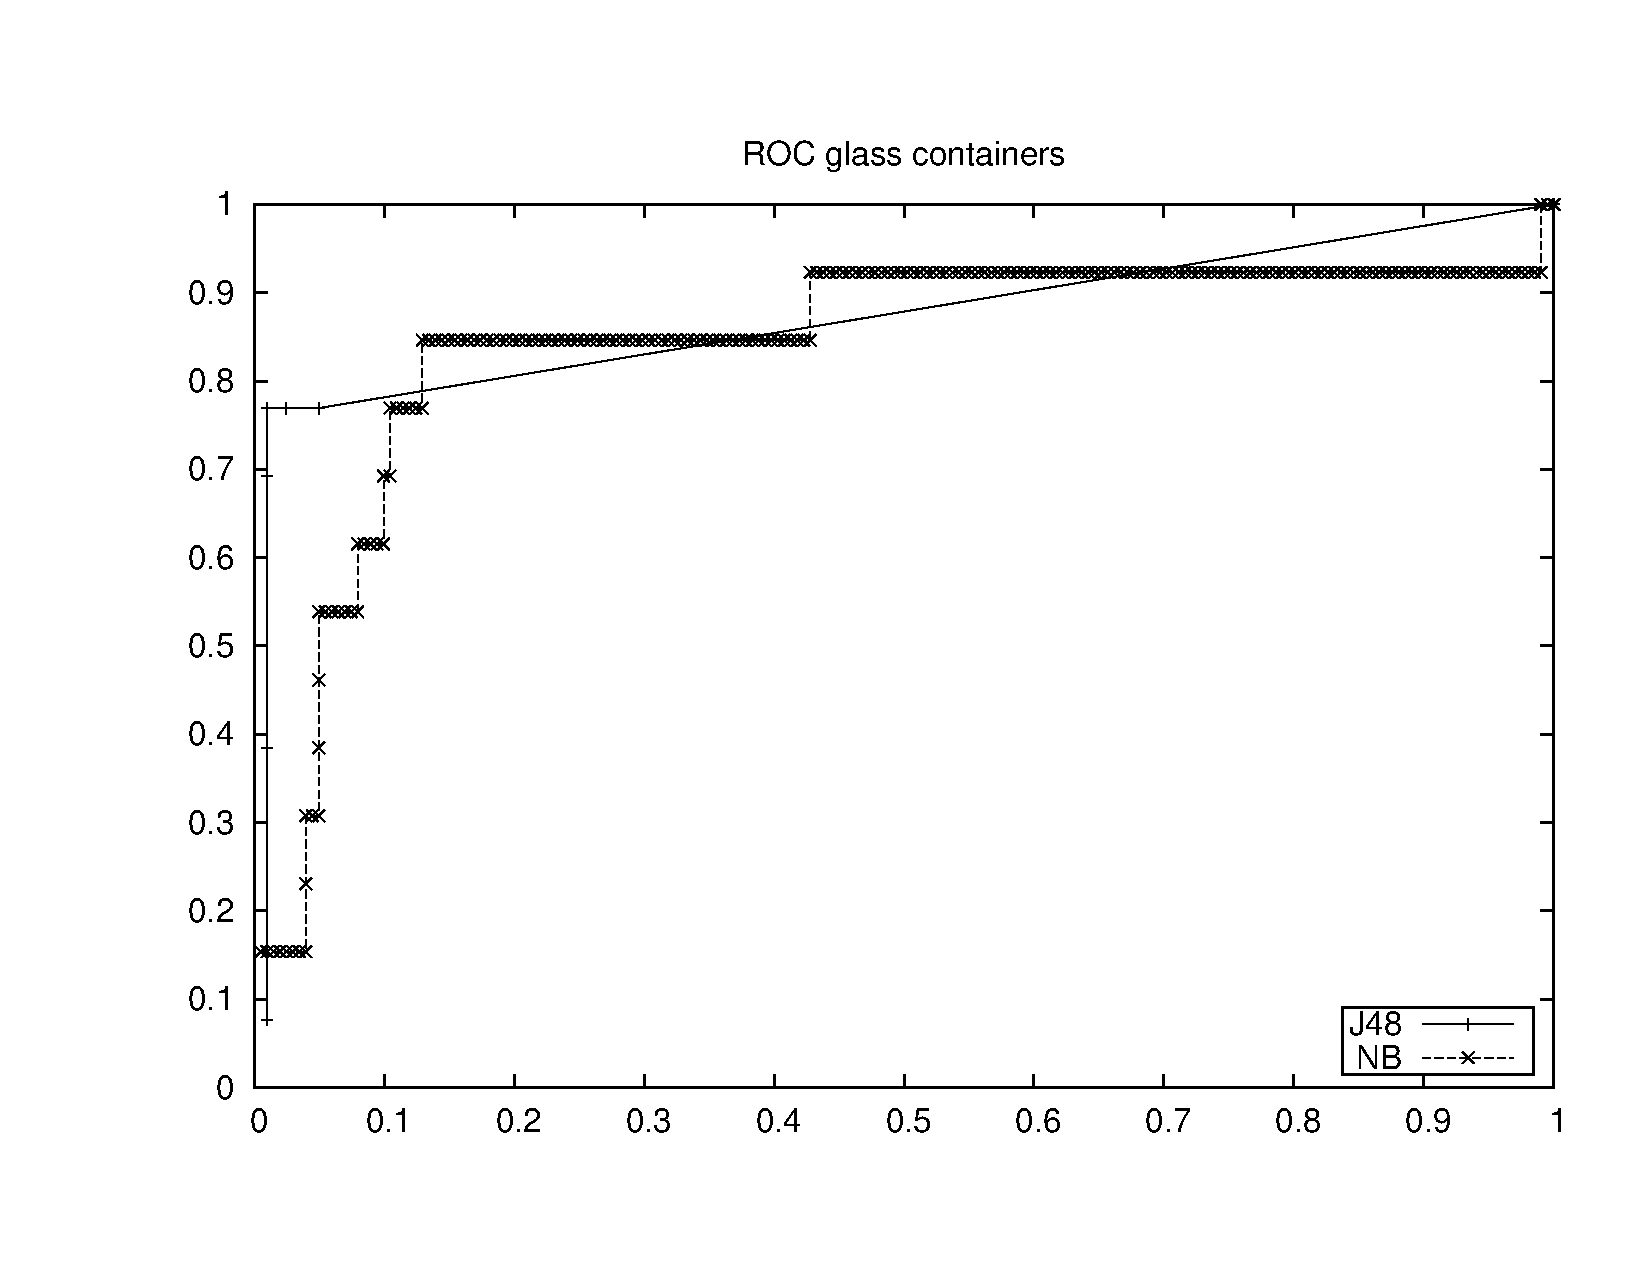
\includegraphics[height=3in]{pics/a3/ROC_glass_containers.pdf}
	\caption{ROC-Kurve f\"ur \emph{Naive Bayes} und \emph{J48} \"uber das Attribut \emph{containers}}
\end{figure}

\begin{figure}[htbp]
	\centering
		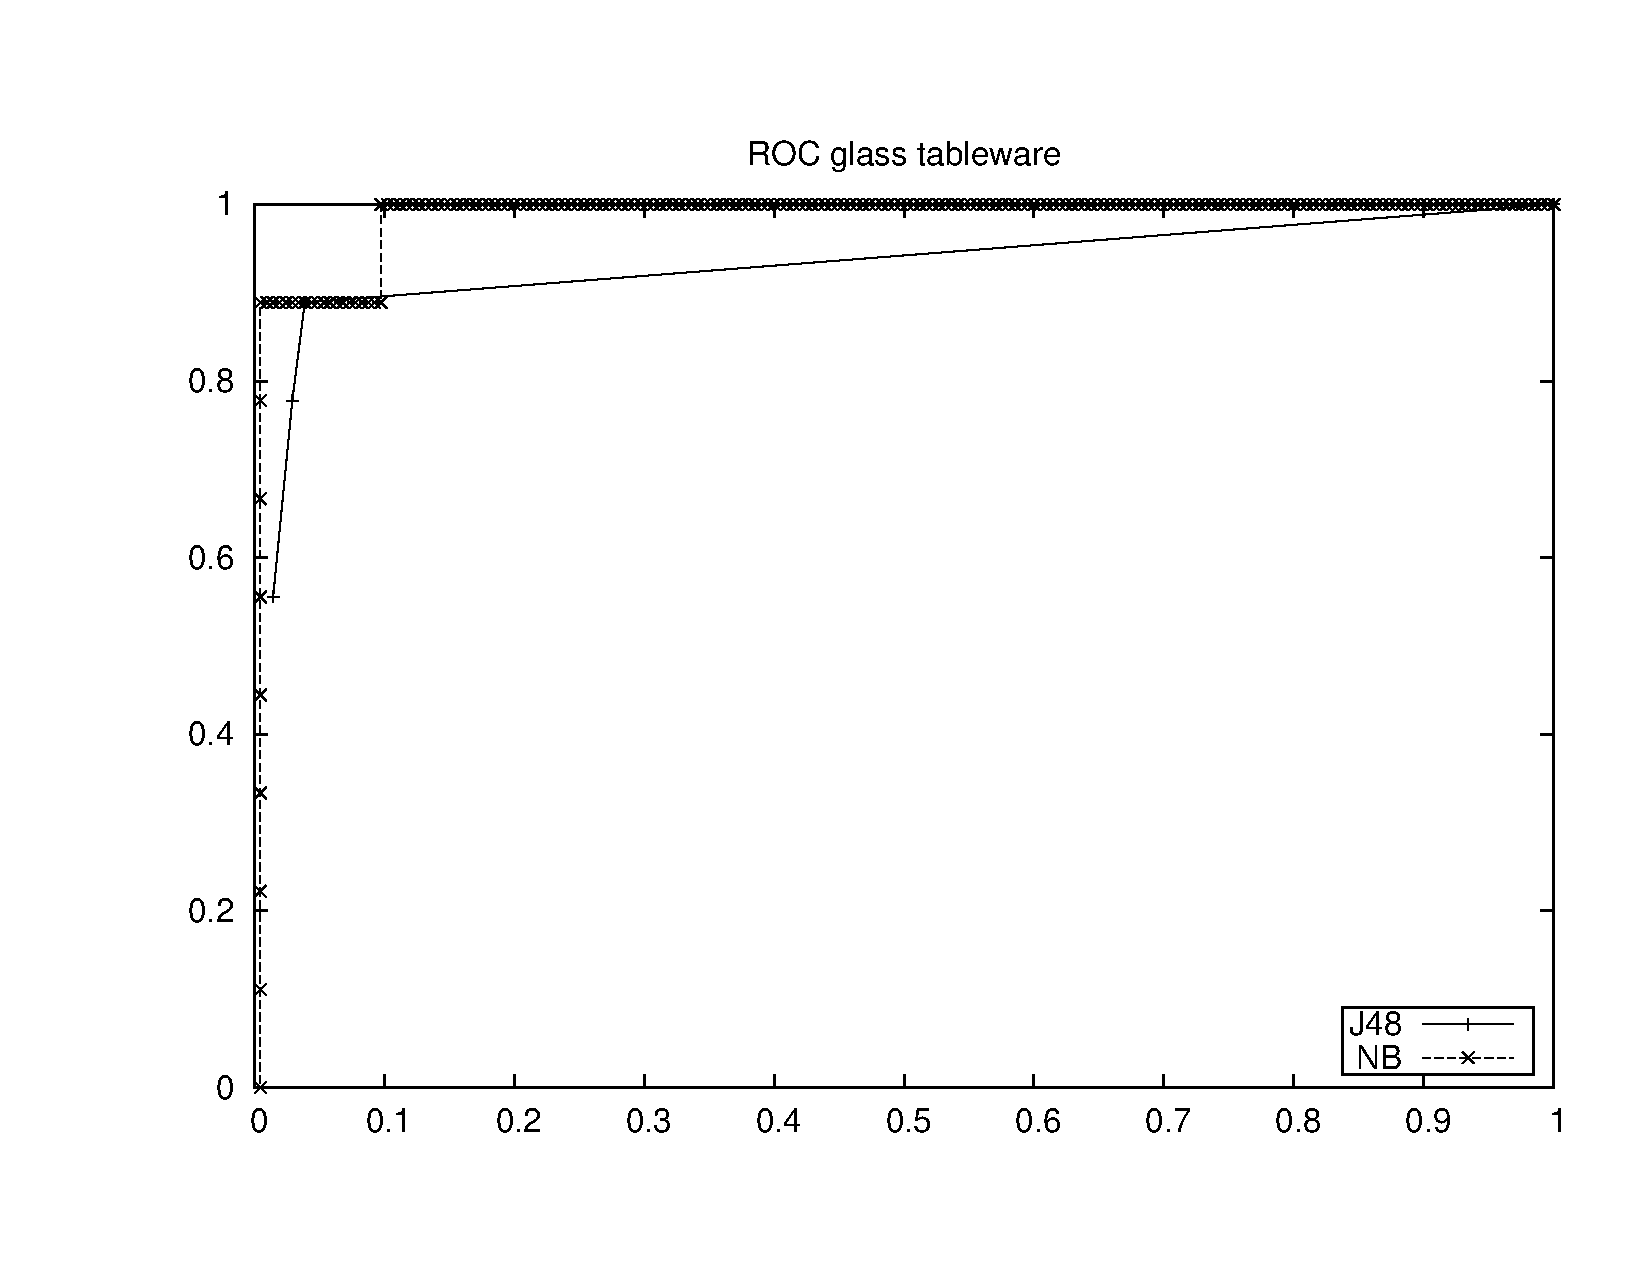
\includegraphics[height=3in]{pics/a3/ROC_glass_tableware.pdf}
	\caption{ROC-Kurve f\"ur \emph{Naive Bayes} und \emph{J48} \"uber das Attribut \emph{containers}}
\end{figure}

Bis auf wenige Klassen hat \emph{J48} eine h\"ohere Fl\"ache unter der ROC Kurve.
Anhand der ROC Kurven kann man also sagen, dass f\"ur eine uniforme Klassenverteilung und f\"ur eine Verteilung mit mehr negativen als positiven Beispielen \emph{J48} bessere Ergebnisse liefert. Bei Besonders vielen positiven Beispielen k\"onnte der Naive Bayes Klassifizierer bessere Ergebnisse erzielen.

\newpage
\section*{Aufgabe 4 Entscheidungsb\"aume}

Datensets: glass (discretize filter), kr-vs-kp

\textbf{Area under ROC curve}

\begin{tabular}{c|c|c|c|c|c|c}
				Regellerner       & \emph{bwf} & \emph{bwn} & \emph{vwf}  & \emph{cont} & \emph{table} & \emph{head} \\ \hline
				\emph{J48 - unpruned}& 0.73 & 0.70 & 0.71 & 0.87 & 0.92 & 0.92 \\ \hline
				\emph{J48 - pruned}  & 0.77 & 0.73 & 0.73 & 0.86 & 0.87 & 0.84 \\ \hline
				\emph{ID3}           & 0.62 & 0.70 & 0.59 & 0.81 & 0.77 & 0.88 \\ \hline
\end{tabular}

Pruning hat nichts gebracht!

\begin{tabular}{c|c|c|c}
				Regellerner       & \emph{won} & \emph{nowin} \\ \hline
				\emph{J48 - unpruned} & 1.0 & 1.0  \\ \hline
				\emph{J48 - pruned}  & 1.0 & 1.0  \\ \hline
				\emph{ID3}  & 1.0 & 1.0 \\ \hline
\end{tabular}


\textbf{Accuracy}

\begin{tabular}{c|c|c}
				Regellerner       & \emph{glass} & \emph{kr-vs-kp}  \\ \hline
				\emph{J48 - unpruned}  & 57.94 & 99.41 \\ \hline
				\emph{J48 - pruned} & 57.94  & 99.44 \\ \hline
				\emph{ID3}  & 50.47 & 99.69\\ \hline
\end{tabular}

\textbf{Gr\"osse der entstandenen B\"aume}

\emph{glass}:
\begin{tabular}{c|c|c}
	Regellerner       & \emph{size of the tree} & \emph{number of leaves}  \\ \hline
	\emph{J48 - unpruned} & 221  & 199  \\ \hline
	\emph{J48 - pruned}   & 81   & 73   \\ \hline
	\emph{ID3}            & 550  & 496  \\ \hline
\end{tabular}


\emph{kr-vs-kp}:
\begin{tabular}{c|c|c}
	Regellerner       & \emph{size of the tree} & \emph{number of leaves}  \\ \hline
	\emph{J48 - unpruned}  & 82 & 43 \\ \hline
	\emph{J48 - pruned} & 59  & 31 \\ \hline
	\emph{ID3}  & 95 & 49\\ \hline
\end{tabular}

Betrachtet man die Fl\"ache unter der ROC Kurve so hat \emph{ID3} im Allgemeinen schlechtere Werte. Dies spiegelt sich auch in der Accuracy wieder. Au\ss erdem erzeugt \emph{ID3} immer einen gr\"o\ss eren Baum. Man kann also deutlich erkennen, das ein gro\ss er Baum schlecht veralgemeinert und somit auch schlechtere Performancewerte erzielt. Das Pruning von \emph{J48} erzeugt einen kleineren Baum, der allerdings nicht deutlich bessere Performance liefert. Dieser Effekt ist dabei wahrscheinlich stark abh\"angig von den von uns gew\"ahlten Datensets.
\newpage
\section*{Aufgabe 5 Nearest Neighbour}

\textbf{Accuracy}

\begin{table}[htb]
	\centering
\begin{tabular}{c|c|c}
                \emph{k-NN}       & \emph{glass} & \emph{kr-vs-kp}  \\ \hline
				\emph{k = 1}  & 59.35  & 96.28  \\ \hline
				\emph{k = 3}  & 57.01  & 96.50  \\ \hline
				\emph{k = 5}  & 58.88  & 96.03  \\ \hline
				\emph{k = 7}  & 57.01  & 95.40  \\ \hline
				\emph{k = 9}  & 56.07  & 95.24  \\ \hline
				\emph{k = 11} & 56.07  & 95.06  
\end{tabular}
\end{table}

H\"ochste cross validation performance liegt bei $k = 1$ bzw $k = 3$. Damit ist der \emph{k-NN} Klassifizierer f\"ur den \emph{glass} Datensatz besser und f\"ur den \emph{kr-vs-kp} Datensatz schlechter als die Entscheidungsbaumlerner.




\newpage
\section*{Aufgabe 6 Regressionsb\"aume}


Tabelle f\"ur den \emph{Mean Absolute Error}:

\begin{table}
\begin{tabular}{c|c|c|c|c}
Datensatz  & \emph{R P MAE } & \emph{R U MAE} & \emph{M P MAE} & \emph{M U MAE} \\ \hline
\emph{auto-price}  & 2096.37 & 2075.07& 1403.20 & 1466.56 \\ \hline
\emph{concrete}    & 6.77    & 6.48   & 4.27    & 4.74     \\ \hline
\emph{housing}     & 3.29    & 3.20   & 2.39    & 2.50     \\ \hline
\emph{stock}       & 1.19    & 1.17   & 0.67    & 0.67     \\ \hline
\emph{winequality} & 0.55    & 0.53   & 0.51    & 0.55       
\end{tabular}
\caption{R: \emph{Regression-Trees} or M: \emph{Model-Trees} \\
U: \emph{unpruned} or P: \emph{pruned} }
\end{table}


Tabelle für den \emph{Root Mean Squared Error}:

\begin{table}
\begin{tabular}{c|c|c|c|c}
Datensatz  & \emph{R P RMSE} & \emph{R U RMSE} & \emph{M P RMSE} & \emph{M U RMSE} \\ \hline
\emph{auto-price}  & 3336.37  & 3287.12 & 2094.59 & 2171.16 \\ \hline
\emph{concrete}    & 8.68 & 8.33 & 5.89 & 6.36 \\ \hline
\emph{housing}     & 4.82 & 4.72 & 3.71 & 3.75 \\ \hline
\emph{stock}       & 1.60 & 1.59 & 0.93 & 0.94 \\ \hline
\emph{winequality} & 0.72 & 0.70 & 0.68 & 0.71   
\end{tabular}
\caption{R: \emph{Regression-Trees} or M: \emph{Model-Trees} \\
U: \emph{unpruned} or P: \emph{pruned} }
\end{table}


Aus den Tabellen k\"onnen wir ablesen, dass bei Regression-Tasks keine Verbesserung bringt. \emph{Model-Trees} haben auf allen Datens\"atze einen kleineren Fehler als \emph{Regression-Trees}. Verwendet man Pruning bei \emph{Model-Trees} liefert es eine leichte Verbesserung.


\emph{M5P} liefert einen dem aus der \"Ubung \"ahnlichen Baum: Auf den ersten beiden Ebenen wird an denselben Attributen gesplittet. Danach erzeugt \emph{M5P} direkt Bl\"atter und l\"ost den Baum  nicht feiner auf. Der \emph{M5P}-Baum ist kleiner und wahrscheinlich allgemeiner. 

Der \emph{Root Mean Squared Error} des Baumes aus der \"Ubung betrugt $0.75$, der jetzt gelernte Baum hat einen \emph{RMSE} von $0.64$ auf den Testdaten. Dies best\"atigt unsere Vermutung, dass der \emph{M5P}-Baum allgemeiner ist.
\newpage
\section*{Aufgabe 7 Ensemble-Lernen}
%!TEX root = main.tex
\textbf{Performance Normal} \\
\begin{tabular}{l|c|c|c|c|c}
	             & yeast & vowel & vehicle &  sick & abalone  \\ \hline
J48              &  56.0 &  81.5 &  72.5   &  98.9 & 21.2     \\ 
\end{tabular}\\ \\


\textbf{Performance Bagging} \\
\begin{tabular}{l|c|c|c|c|c}
Iterations       & yeast & vowel & vehicle &  sick & abalone     \\ \hline
10               &  60.8 & 90.4  &  76.6   & 98.7  &  23.1       \\ \hline
20               &  61.0 & 91.3  &  75.9   & 98.9  &  23.2       \\ \hline
50               &  62.0 & 91.9  &  76.2   & 98.9  &  23.5       \\ \hline
100              &  61.3 & 92.5  &  76.0   & 98.8  &  23.5       \\ 
\end{tabular}\\ \\

\textbf{Performance AdaBoost} \\
\begin{tabular}{l|c|c|c|c|c}
Iterations       & yeast & vowel & vehicle &  sick & abalone     \\ \hline
10               & 56.4  &  93.3 &  76.2   &  99.2 &  21.7       \\ \hline
20               & 58.1  &  95.9 &  77.0   &  99.2 &  21.9       \\ \hline
50               & 58.9  &  96.0 &  78.4   &  99.2 &  22.6       \\ \hline
100              & 58.6  &  96.5 &  78.8   &  99.0 &  22.7       \\ 
\end{tabular}\\ \\


\textbf{Performance Random Forests} \\
\begin{tabular}{l|c|c|c|c|c}
Number of Trees  & yeast & vowel & vehicle &  sick & abalone     \\ \hline
10               & 57.9  & 96.0  & 77.0    &  98.4 &  22.4       \\ \hline
20               & 61.2  & 98.0  & 76.5    &  98.4 &  23.4       \\ \hline
50               & 61.3  & 98.2  & 76.7    &  98.5 &  23.4       \\ \hline
100              & 61.4  & 98.5  & 76.5    &  98.4 &  23.8       \\ 
\end{tabular}\\ \\

Generell verbessern alle 3 Ensemble Lerner die Performance gegen\"uber dem regulären \emph{J48}. Bei \emph{Bagging} bringt eine erh\"ohte Anzahl der Iteration nur sehr geringe Verbesserungen auf unseren Datensets. Durch \emph{Boosting} kann die Performance um mehrere Prozent steigen, wenn man die Zahl der Iterationen erh\"oht. Bei \emph{Random Forests} h\"angt eine Steigerung der Performance durch eine erh\"ohte Anzahl von Trees stark vom Datensatz ab. 

\newpage
\section*{Aufgabe 8 Entdecken von Assoziationsregeln}

numerische attribute entfernt: fnlwgt, education-num

andere attribute entfernt: marital-status, capital-gain, capital-loss, sex

sortiert nach lift: 

relationship=Not-in-family 12583 ==> class=<=50K 11307    conf:(0.9) < lift:(1.18)> lev:(0.04) [1734] conv:(2.36)



numerische attribute entfernt: fnlwgt, education-num

andere attribute entfernt: marital-status, capital-gain, capital-loss, sex, age, relationship, native-country

sortiert nach confidence:

class=>50K 11687 ==> race=White 10607    conf:(0.91)

Da 85 \% der Teilnehmer der Studie race = white hatten, wurden sehr viele Regeln der Form ? => race = white gefunden. Entfernt man dieses Attribut, findet man interessantere Regeln.


attributes \u"brig: age, education, marital-status, occupation

1. age=0 9627 ==> marital-status=Never-married 8229    conf:(0.85)

2. age=3 8296 ==> marital-status=Married-civ-spouse 5139    conf:(0.62)


attributes: marital-status, relationship, class

class=>50K 11687 ==> marital-status=Married-civ-spouse 9984    conf:(0.85)

relationship=Own-child 7581 ==> class=<=50K 7470    conf:(0.99)





%TODO verschoenern
\newpage
\section*{Aufgabe 9  Pre-Processing}
%!TEX root = main.tex
Datensets: ionosphere, iris, yeast, letter.

Accuracy
\begin{tabular}{l|c|c|c|c}
	               & ionosphere & iris  & yeast & letter \\ \hline
J48 unfiltered     &  91.5      &  96.0 &  56.0 &  88.0  \\ \hline
J48 filtered       &  89.2      &  94.0 &  59.1 &  78.6  \\ \hline
FilteredClassifier &  91.2      &  93.3 &  57.0 &  78.7  \\ \hline
\end{tabular}\\ \\

Number of Leaves
\begin{tabular}{l|c|c|c|c}
	               & ionosphere & iris  & yeast & letter \\ \hline
J48 unfiltered     &  18        &  5    &  185  &  1226  \\ \hline
J48 filtered       &  21        &  3    &  64   &  9624  \\ \hline
FilteredClassifier &  21        &  3    &  64   &  9624  \\ \hline
\end{tabular}\\ \\



\end{document}
